% Created 2020-10-16 Fri 17:37
% Intended LaTeX compiler: pdflatex
\documentclass[presentation]{beamer}
\usepackage[utf8]{inputenc}
\usepackage[T1]{fontenc}
\usepackage{graphicx}
\usepackage{grffile}
\usepackage{longtable}
\usepackage{wrapfig}
\usepackage{rotating}
\usepackage[normalem]{ulem}
\usepackage{amsmath}
\usepackage{textcomp}
\usepackage{amssymb}
\usepackage{capt-of}
\usepackage{hyperref}
\usetheme{UoB}
\author{Mark Blyth}
\date{\textit{[2020-10-26 Mon]}}
\title{BSplines for CBC discretisation}
\hypersetup{
 pdfauthor={Mark Blyth},
 pdftitle={BSplines for CBC discretisation},
 pdfkeywords={},
 pdfsubject={},
 pdfcreator={Emacs 27.1 (Org mode 9.3)}, 
 pdflang={English}}
\begin{document}

\maketitle

\section{Intro}
\label{sec:orgabc4901}
\begin{frame}[label={sec:org48e901b}]{Last time}
Proposals for project ideas, with a focus on
\vfill
\begin{itemize}
\item Efficiency
\begin{itemize}
\item Avoiding high-dimensional discretisation
\item Producing fast prediction/correction steps
\end{itemize}
\end{itemize}
\vfill
\begin{itemize}
\item Noise-robustness
\begin{itemize}
\item Finding continuation solutions in the face of measurement noise
\item Whether or not to consider stochasticity
\end{itemize}
\end{itemize}
\end{frame}

\begin{frame}[label={sec:org9f37fcc}]{This time}
Preliminary results for efficient splines-based discretisation
\vfill
\begin{itemize}
\item Replace Fourier discretisation with splines discretisation
\begin{itemize}
\item Goal: more noise-robust, lower dimensional
\end{itemize}
\end{itemize}
\vfill
\begin{itemize}
\item Was facing issues with numerical simulations
\end{itemize}
\vfill
\begin{itemize}
\item New results from Friday: it works!
\end{itemize}
\end{frame}

\section{Using BSplines}
\label{sec:org7ae0f07}
\begin{frame}[label={sec:org5aba726}]{Spline models}
Currently testing spline discretisation; what is this?
\vfill
\begin{itemize}
\item Standard continuation: set up a BVP for a PO
\begin{itemize}
\item Continuation vector encodes discretised solution + regularisation constraints
\item Orthogonal collocation usually used
\end{itemize}
\end{itemize}
\vfill
\begin{itemize}
\item Control-based continuation: set up a variational problem
\begin{itemize}
\item Find a non-invasive control target
\item Use a solving algo on discretised signals
\end{itemize}
\end{itemize}
\vfill
\begin{itemize}
\item Splines are maximally smooth piecewise-polynomial models
\begin{itemize}
\item BSplines form a set of basis functions for spline models
\item BSpline coefficients are used as signal discretisation
\end{itemize}
\end{itemize}
\end{frame}

\begin{frame}[label={sec:orgc01ad02}]{The BSpline method}
Key goal: noninvasive control
\begin{itemize}
\item For proportional control, zero tracking error means zero control action
\item Noninvasive \(\iff\) system output matches control target
\end{itemize}
\vfill
Algo summary:
\begin{itemize}[<+->]
\item Produce two initial discretisations by running the system uncontrolled
\item Use secant pseudo-arclength continuation to track solution under parameter change
\begin{enumerate}
\item Extract discretisation from continuation vector
\item Translate discretisation into a control target
\item Run the system with that target
\item Discretise the output
\item Newton-solve for discretised input = discretised output
\item Repeat across target parameter range
\end{enumerate}
\end{itemize}
\end{frame}

\section{BSpline results + where the dragons be}
\label{sec:org7fabf48}

\begin{frame}[label={sec:org8179fb4}]{Results}
\begin{center}
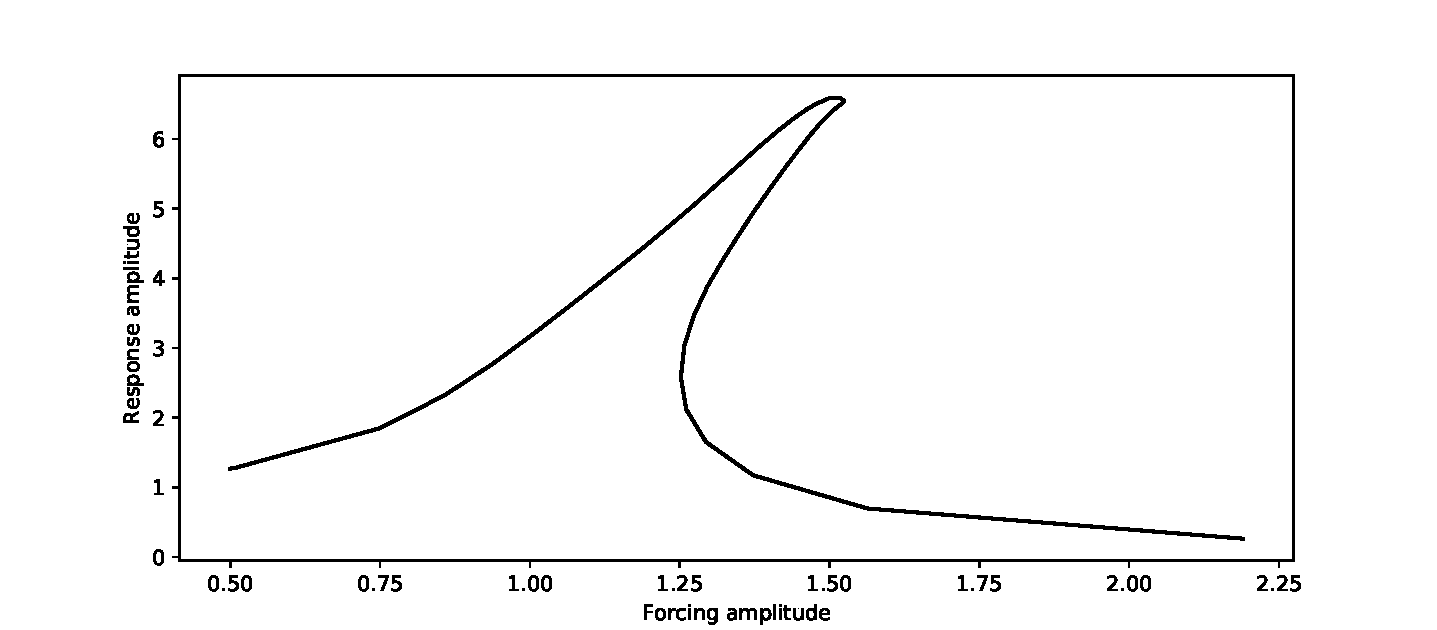
\includegraphics[width=.9\linewidth]{./success.pdf}
\end{center}

It works!
\end{frame}

\begin{frame}[label={sec:orgfe3828f}]{Results}
\begin{itemize}
\item Results are for a harmonically forced Duffing oscillator
\begin{itemize}
\item Validation: an solve analtically for frequency-response curves
\item Simplicity: system output is easy to Fourier- and spline-discretise
\end{itemize}
\end{itemize}
\vfill
\begin{itemize}
\item Analytic results need computing through continuation
\begin{itemize}
\item For simplicity I didn't take the continuation route
\item That's coming next!
\end{itemize}
\end{itemize}
\end{frame}

\begin{frame}[label={sec:orgff4639a}]{Results}
\begin{center}
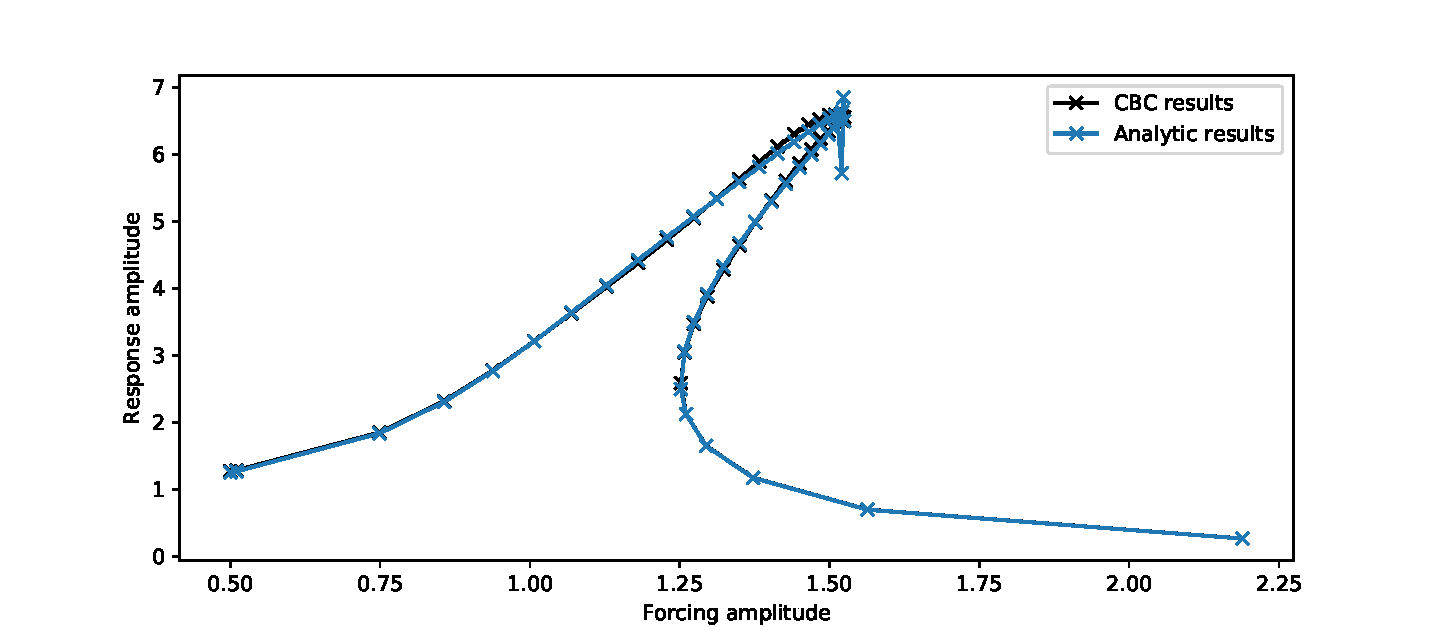
\includegraphics[width=.9\linewidth]{./comparison.pdf}
\end{center}

It works!
\end{frame}

\begin{frame}[label={sec:org05f48f0}]{The hard parts}
\begin{itemize}
\item All spline curves require exterior knots
\begin{itemize}
\item `Extra' control points placed outside the range of the data
\item Allows the spline curve to fit the data endpoints
\end{itemize}
\end{itemize}
\vfill
\begin{itemize}
\item Periodic splines require careful treatment
\begin{itemize}
\item Coefficient vectors have a special structure
\item Perturbations (prediction steps, finite differences) break that structure
\item Can make the coefficient vectors perturbation-robust quite easily, but it requires custom code
\end{itemize}
\end{itemize}
\vfill
\begin{itemize}
\item Periodic splines take periodic exterior knots, and periodic coefficients for exterior BSplines
\begin{itemize}
\item First \(k\) coeff's must equal last \(k\) coeffs
\item This is easy to handle; SciPy tries to be very general, and ends up handling it badly
\end{itemize}
\end{itemize}
\end{frame}

\begin{frame}[label={sec:org517b0cf}]{The hard parts}
My Newton solver doesn't solve the continuation equations very well
\vfill
\begin{itemize}
\item Accepted solution vectors don't accurately solve the system
\begin{itemize}
\item Convergence declared when solution stops changing
\item Converged vector gives a solution error of \(\mathcal{O}(10^{-1})\)
\end{itemize}
\end{itemize}
\vfill
\begin{itemize}
\item My DIY solver `jumps'
\begin{itemize}
\item Solution vector normally takes small parameter-steps
\item Newton solver causes solution to take a very big parameter step, to somewhere wrong
\end{itemize}
\end{itemize}
\vfill
\begin{itemize}
\item SciPy solvers overcome this\ldots{}
\begin{itemize}
\item \ldots{}however SciPy quasi-Newton solvers have the same issue!
\item Other methods work very well, but they're a black box
\item No idea what they're doing, or how or why
\end{itemize}
\end{itemize}
\end{frame}

\begin{frame}[label={sec:orgeade945}]{Jumping solutions}
\begin{center}
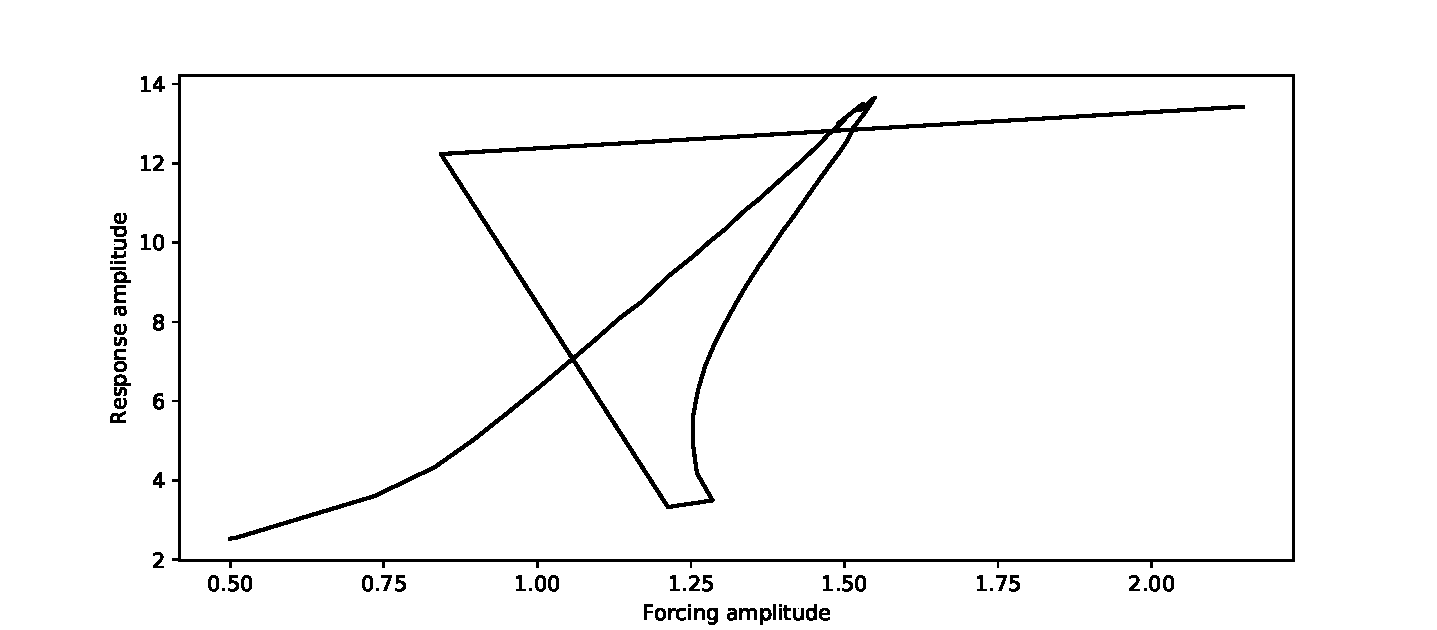
\includegraphics[width=.9\linewidth]{./jump.pdf}
\end{center}

(Actually using slightly older code, but same results apply)
\end{frame}

\section{Existence and uniqueness [main question]}
\label{sec:orgec175d5}
\begin{frame}[label={sec:org9954c77}]{Solution existence and uniqueness}
Under what conditions can we guarantee a solution to the CBC equations exists?
\begin{itemize}
\item Undiscretised case: solution definitely exists
\begin{itemize}
\item Infinite Fourier discretisation is an exact representation of continuous case; solution must exist
\item Trucated Fourier is equivalent to infinite Fourier up to computational precision; solution \emph{probably} exists
\end{itemize}
\end{itemize}
\vfill
Solution to discretised equations must exist when discretisation is exact
\begin{itemize}
\item Can't guarantee splines are exact; how do we know if a solution exists?
\end{itemize}
\vfill
Generally, when can we guarantee discretising won't cause the system to become unsolvable?
\end{frame}

\section{Next steps}
\label{sec:org642c013}
\begin{frame}[label={sec:org2906932}]{Next steps}
\begin{enumerate}
\item Testing spline discretisation more
\begin{itemize}
\item Try it out on a neuron model
\item Try to break it!
\end{itemize}
\end{enumerate}
\vfill
\begin{enumerate}
\item Understand the solver issues
\begin{itemize}
\item Solvers are clearly crucial to good results
\item Need to understand where the Newton problems are coming from
\end{itemize}
\end{enumerate}
\vfill
\begin{enumerate}
\item Compare splines to other methods
\begin{itemize}
\item Compare to Fourier, wavelets, collocation
\item Compare in terms of noise-robustness, efficiency, achievable accuracy, ease of use
\end{itemize}
\end{enumerate}
\end{frame}
\end{document}
